%% Преамбула TeX-файла

% 1. Стиль и язык
\documentclass[utf8x]{G7-32} % Стиль (по умолчанию будет 14pt)
\usepackage[T2A]{fontenc}
\usepackage[russian]{babel}
% Остальные стандартные настройки убраны в preamble.inc.tex.
%%==========================================%%
%% Для избежания переносов слов
\usepackage{ragged2e}
\usepackage{microtype}

\justifying
\sloppy
\tolerance=500
\hyphenpenalty=10000
\emergencystretch=3em
%%==========================================%%

% Настройки стиля ГОСТ 7-32
% Для начала определяем, хотим мы или нет, чтобы рисунки и таблицы нумеровались в пределах раздела, или нам нужна сквозная нумерация.
\EqInChapter % формулы будут нумероваться в пределах раздела
\TableInChapter % таблицы будут нумероваться в пределах раздела
\PicInChapter % рисунки будут нумероваться в пределах раздела

% Добавляем гипертекстовое оглавление в PDF
\usepackage[
bookmarks=true, colorlinks=true, unicode=true,
urlcolor=black,linkcolor=black, anchorcolor=black,
citecolor=black, menucolor=black, filecolor=black,
]{hyperref}

%Величина «красной строки»


\usepackage[tableposition=top,singlelinecheck=false]{caption}
%\usepackage{subcaption}

\DeclareCaptionLabelFormat{gostfigure}{Рисунок #2}
\DeclareCaptionLabelFormat{gosttable}{Таблица #2}
\DeclareCaptionLabelSeparator{gost}{~---~}
% Можно разбивать длинные таблицы вручную, оформляя каждую как table. В этом случае для продолжений таблицы нужно создать отдельный стиль заголовка
\DeclareCaptionLabelFormat{continued}{Продолжение таблицы~#2}
\captionsetup*[ContinuedFloat]{labelformat=continued}
\captionsetup{labelsep=gost}
\captionsetup*[figure]{labelformat=gostfigure, justification=centering,font={small, bf}}  % выравнивание по центру
\captionsetup*[table]{hangindent=-10pt, indention=0pt,parindent=0pt,margin=0pt,labelformat=gosttable,justification=raggedright,font={small,it}}
\captionsetup*[lstlisting]{font={small, it}}

% Изменение начертания шрифта --- после чего выглядит таймсоподобно.
% apt-get install scalable-cyrfonts-tex

\IfFileExists{cyrtimes.sty}
    {
        \usepackage{cyrtimespatched}
    }
    {
        % А если Times нету, то будет CM...
    }

\usepackage{graphicx}   % Пакет для включения рисунков
%расположение графики
\graphicspath{{images/}{figures/}{screnshots/}{../images/}}  % папки с картинками

% С такими оно полями оно работает по-умолчанию:
% \RequirePackage[left=20mm,right=10mm,top=20mm,bottom=20mm,headsep=0pt]{geometry}
% Если вас тошнит от поля в 10мм --- увеличивайте до 20-ти, ну и про переплёт не забывайте:
\geometry{right=10mm}
\geometry{left=30mm}


% Пакет Tikz
\usepackage{tikz}
\usetikzlibrary{arrows,positioning,shadows}

% Произвольная нумерация списков.
\usepackage{enumerate}

% ячейки в несколько строчек
\usepackage{multirow}

% itemize внутри tabular
\usepackage{paralist,array}


% Настройки листингов.
% 8 Листинги

\usepackage{listings}

% Значения по умолчанию
\lstset{
  basicstyle= \footnotesize\ttfamily,
  breakatwhitespace=true,% разрыв строк только на whitespacce
  breaklines=true,       % переносить длинные строки
%   captionpos=b,          % подписи снизу -- вроде не надо
  inputencoding=koi8-r,
  numbers=left,          % нумерация слева
  numberstyle=\footnotesize,
  showspaces=false,      % показывать пробелы подчеркиваниями -- идиотизм 70-х годов
  showstringspaces=false,
  showtabs=false,        % и табы тоже
  stepnumber=1,
  tabsize=4,              % кому нужны табы по 8 символов?
  frame=single
}

% Стиль для псевдокода: строчки обычно короткие, поэтому размер шрифта побольше
\lstdefinestyle{pseudocode}{
  basicstyle=\small\ttfamily,
  keywordstyle=\color{black}\bfseries\underbar,
  language=Pseudocode,
  numberstyle=\footnotesize,
  commentstyle=\footnotesize\it\texttt
}

% Стиль для обычного кода: маленький шрифт
\lstdefinestyle{realcode}{
  basicstyle=\scriptsize,
  numberstyle=\footnotesize
}

% Стиль для коротких кусков обычного кода: средний шрифт
\lstdefinestyle{simplecode}{
  basicstyle=\footnotesize,
  numberstyle=\footnotesize
}

% Стиль для BNF
\lstdefinestyle{grammar}{
  basicstyle=\footnotesize,
  numberstyle=\footnotesize,
  stringstyle=\bfseries\ttfamily,
  language=BNF
}

% Определим свой язык для написания псевдокодов на основе Python
\lstdefinelanguage[]{Pseudocode}[]{Python}{
  morekeywords={each,empty,wait,do},% ключевые слова добавлять сюда
  morecomment=[s]{\{}{\}},% комменты {а-ля Pascal} смотрятся нагляднее
  literate=% а сюда добавлять операторы, которые хотите отображать как мат. символы
    {->}{\ensuremath{$\rightarrow$}~}2%
    {<-}{\ensuremath{$\leftarrow$}~}2%
    {:=}{\ensuremath{$\leftarrow$}~}2%
    {<--}{\ensuremath{$\Longleftarrow$}~}2%
}[keywords,comments]

% Свой язык для задания грамматик в BNF
\lstdefinelanguage[]{BNF}[]{}{
  morekeywords={},
  morecomment=[s]{@}{@},
  morestring=[b]",%
  literate=%
    {->}{\ensuremath{$\rightarrow$}~}2%
    {*}{\ensuremath{$^*$}~}2%
    {+}{\ensuremath{$^+$}~}2%
    {|}{\ensuremath{$|$}~}2%
}[keywords,comments,strings]

% Подписи к листингам на русском языке.
\renewcommand\lstlistingname{\cyr\CYRL\cyri\cyrs\cyrt\cyri\cyrn\cyrg}
\renewcommand\lstlistlistingname{\cyr\CYRL\cyri\cyrs\cyrt\cyri\cyrn\cyrg\cyri}


% Полезные макросы листингов.
% Любимые команды
\newcommand{\Code}[1]{\textbf{#1}}


\renewcommand{\rmdefault}{ftm}

\begin{document}

\frontmatter % выключает нумерацию ВСЕГО; здесь начинаются ненумерованные главы: реферат, введение, глоссарий, сокращения и прочее.

% Команды \breakingbeforechapters и \nonbreakingbeforechapters
% управляют разрывом страницы перед главами.
% По-умолчанию страница разрывается.

% \nobreakingbeforechapters
% \breakingbeforechapters

%% Также можно использовать \Referat, как в оригинале
\begin{abstract}
Это пример каркаса расчётно-пояснительной записки, желательный к использованию в РПЗ проекта по курсу РСОИ.

Данный опус, как и более новые версии этого документа, можно взять по адресу (\url{https://github.com/rominf/latex-g7-32}).

Текст в документе носит совершенно абстрактный характер.
\end{abstract}

%%% Local Variables: 
%%% mode: latex
%%% TeX-master: "rpz"
%%% End: 


\tableofcontents

\Defines % Необходимые определения. Вряд ли понадобться
\begin{description}
\item[Распределённый] Слово, которое нельзя употреблять. Но надо протестировать длинные строки в глоссарии.
\end{description}

%%% Local Variables:
%%% mode: latex
%%% TeX-master: "rpz"
%%% End:

\Abbreviations %% Список обозначений и сокращений в тексте
\begin{description}
\item [AJAX] Asynchronous Javascript and XML
\item [CLI] Command line interface
\item [DDL] Data Definition Language
\item [DML] Data Manipulation Language
\item [CSS] Cascading Style Sheets
\item [HTML] HyperText Markup Language
\item[SQL] Structured query language.
\item[БД] База данных.
\item[ПО] Программное обеспечение.
\item[СУБД] Система управления базами данных.

\end{description}

%%% Local Variables:
%%% mode: latex
%%% TeX-master: "rpz"
%%% End:


\Introduction

Целью работы является построение логической и физической модели данных выбранной предметной области, освоение навыков работы с программным обеспечением ERwin Data Modeler, ER Assistant, MySQL Workbench, MySQL Server. 

На заключительном этапе работы необходимо представить веб--приложение или полнофункциональное приложение, организующее взаимодействие пользователя с созданной базой данных.  

%\begin{itemize}
%\item проанализировать предложенную ;
%\item спроектировать свою, новую всячину;
%\item изготовить всякую всячину;
%\item проверить её работоспособность.
%\end{itemize}
%
%Вот так-то. А этот абзац вставлен для визуальной оценки отступа от перечня до следующего абзаца.

\mainmatter % это включает нумерацию глав и секций в документе ниже

\newcommand{\erassistant}{ErAssistant~}

\chapter{Построение модели данных}
\label{cha:analysis}
%
% % В начале раздела  можно напомнить его цель
%
В данном разделе описывается процесс создания проекта базы данных в среде \erassistant \textit{(ver. 2.10).}

\section{Работа по методическим указаниям}
Произведем разработку проекта базы данных по теме, утвержденной в рамках дисциплины <<Разработка базы данных>>.
\subsection{Описание предметной области}
Компания занимается производством и продажей небольших статуэток,
раскрашиваемых вручную. Компания имеет несколько производственных
направлений. Миниатюры изготавливаются из гипса, олова или алюминия.

Компания распространяет свои товары по трем каналам. Компания содержит
пять собственных розничных магазинов. Помимо этого, компания владеет
сайтом, на котором ведется online-торговля, и осуществляет оптовые поставки
сторонним
дистрибьюторам.
Для
анализа
статистики,
системой автоматизации производства, нужен интерактивный аналитический
инструмент. Поэтому необходимо спроектировать и построить модель данных,
которая станет хранилищем информации по производству.

В ходе производства изделий система автоматизации производства
управляет всеми станками компании. Каждый станок реализует полный цикл
производства изделий, включая:
\begin{itemize}
	\item заполнение формы сырьем (гипсом, оловом или алюминием);
	\item затвердевание материала;
	\item  удаление изделия из формы после затвердевания;
	\item при необходимости автоматизированная раскраска изделий (оловянные фигурки не раскрашиваются);
	\item сушку после покраски (при необходимости).
\end{itemize}


Покраска и сушка могут производиться за несколько этапов в зависимости
от сложности изделия. По мере готовности изделия проходят проверку,
выполняемую оператором станка.

Оператор станка регистрируется в системе. В ходе этого процесса оператор
сообщает системе автоматизации производства тип производимых изделии и
объем загруженного в машину сырья. Оператор также делает в системе запись
при отбраковке изделий.

В ходе
интервью необходимые для эффективного анализа статистики:
\begin{itemize}
	
	\item  число принятых изделий по объему сырья, видам изделий, машинам и
	\item  время формовки и затвердевания по видам изделий, машинам и дням;
	\item  время покраски и сушки по типам краски, видам изделий, машинам и
	\item  сворачивание по подтипам изделий, которые сворачиваются по типам;
	\item  сворачивание по материалам (гипс, олово или алюминий);
	\item  сворачивание машин по фабрикам, которые сворачиваются по странам;
	\item  сворачивание дней по месяцам, месяцев — по кварталам;
	\item  возможность фильтрации информации по производителю и дате покупки машины.
\end{itemize}

Анализ файла-экспорта из системы автоматизации производства показал,
что для каждого вида производимых изделий есть отдельная строка, в которой
присутствует следующая информация:
\begin{itemize}
	\item  тип изделия;
	\item  объем сырья;
	\item  номер машины;
	\item  личный номер оператора;
	\item  время и дата начала производства (когда серия начата);
	\item  время и дата окончания производства (когда серия закончена);
	\item  флаг отбраковки.
\end{itemize}
%\newpage
\subsection{Построение модели}
По приведенному описанию предметной области построим ее модель в среде \erassistant. Укажем линии связей, назначим им имена, укажем типы и кратность связей. В результате работы, модель примет вид, приведенный на Рисунке \ref{fig:1-metod}.

% TODO: \usepackage{graphicx} required
\begin{figure}[ht]
	\centering
	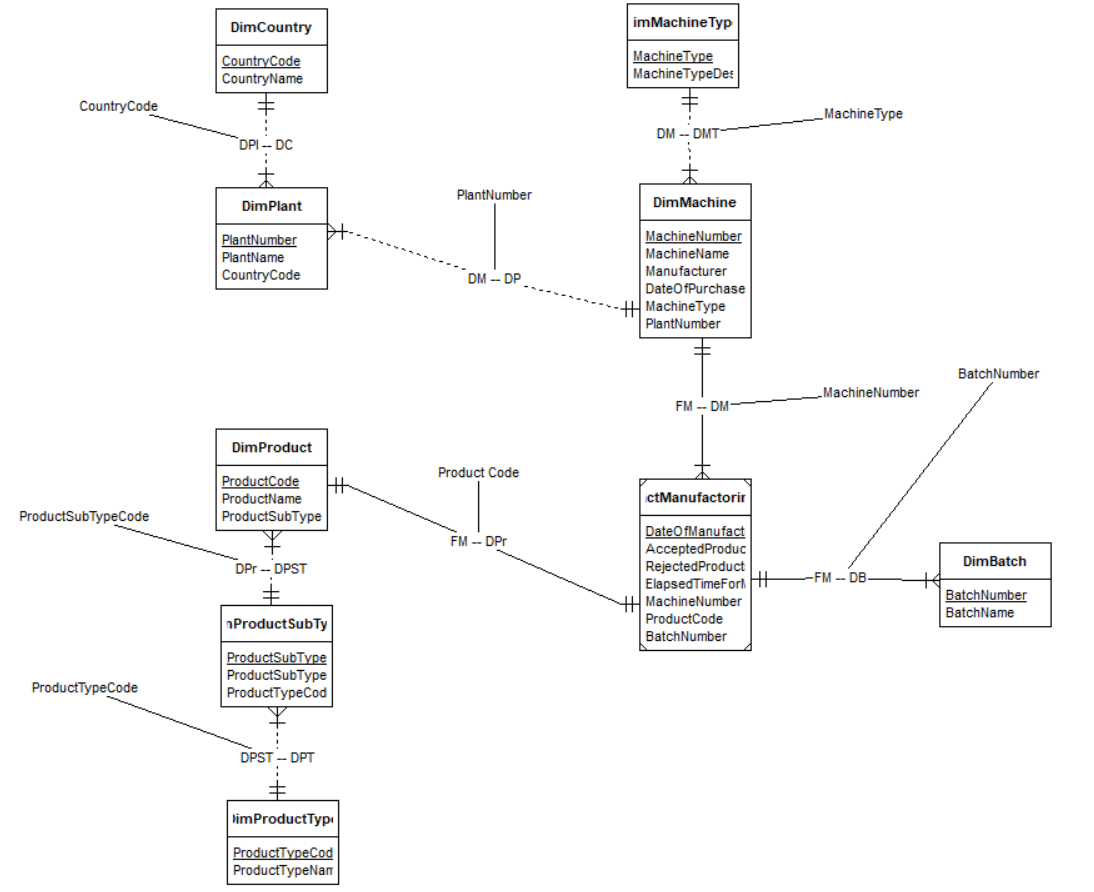
\includegraphics[width=0.9\linewidth]{1-metod}
	\caption{Модель данных Производства со связями}
	\label{fig:1-metod}
\end{figure}
\section{Индивидуальное задание}
Произведем разработку проекта базы данных по индивидуальной теме с использованием программной среды ER Assistant
\subsection{Описание предметной области}
В качестве индивидуального задания была выбрана реализация модели информационной системы по хранению и анализу данных  предприятия, занимающегося сборкой и поставкой спортивных велосипедов для конечных потребителей по индивидуальному заказу.

Предприятие располагает широким выборов компонентов и комплектующих для сборки велосипедов следующих типов:
\begin{itemize}
	\item дорожный;
	\item горный;
	\item кросс-кантри;
	\item эндуро;
	\item прогулочный.
\end{itemize}

Предприятие может предложить сконфигурировать велосипед, отдельно выбрав каждый из предложенных компонентов:
\begin{itemize}
	\item рама;
	\item вилка;
	\item руль;
	\item трансмиссия;
	\item колеса;
	\item тормозная система.
\end{itemize}

Контроль над выполнением работ по сборке велосипеда проводится в виде учета всех операций по сборке, настройке и тестированию, проводимых на территории предприятия ее сотрудниками. При этом каждая запись содержит следующую информацию о проведенных работах:
\begin{itemize}
	\item внутренний номер изделия;
	\item время;
	\item этап работ;
	\item название цеха;
	\item имя мастера;
	\item статус;
	\item примечание.
\end{itemize}

На предприятии ведется учет всех компонентов велосипедов.
В базе данных предприятия хранится информация о каждом компоненте, приобретенном у партнеров или изготовленном самостоятельно.

В независимости от типа компонента он обладает общей информацией о наименовании производителя, месте и времени изготовления, типе и рекомендованной розничной цене. 
Также каждый компонент имеет особые сведения, присущие данному типу детали.

\subsection{Построение модели}
После приведения общих сведений о роде деятельности предприятия, факторизируем модель данных информационной системы предприятия в среде \erassistant (cм Рисунок \ref{fig:1-cycle}). Приложение \erassistant позволяет пользователю создавать, редактировать диаграммы сущностей и связей.

Укажем названия связей, их идентификаторы и кратность, исходя из вида отношений, выстроенных между сущностями.
% TODO: \usepackage{graphicx} required
\begin{figure}[h!]
	\centering
	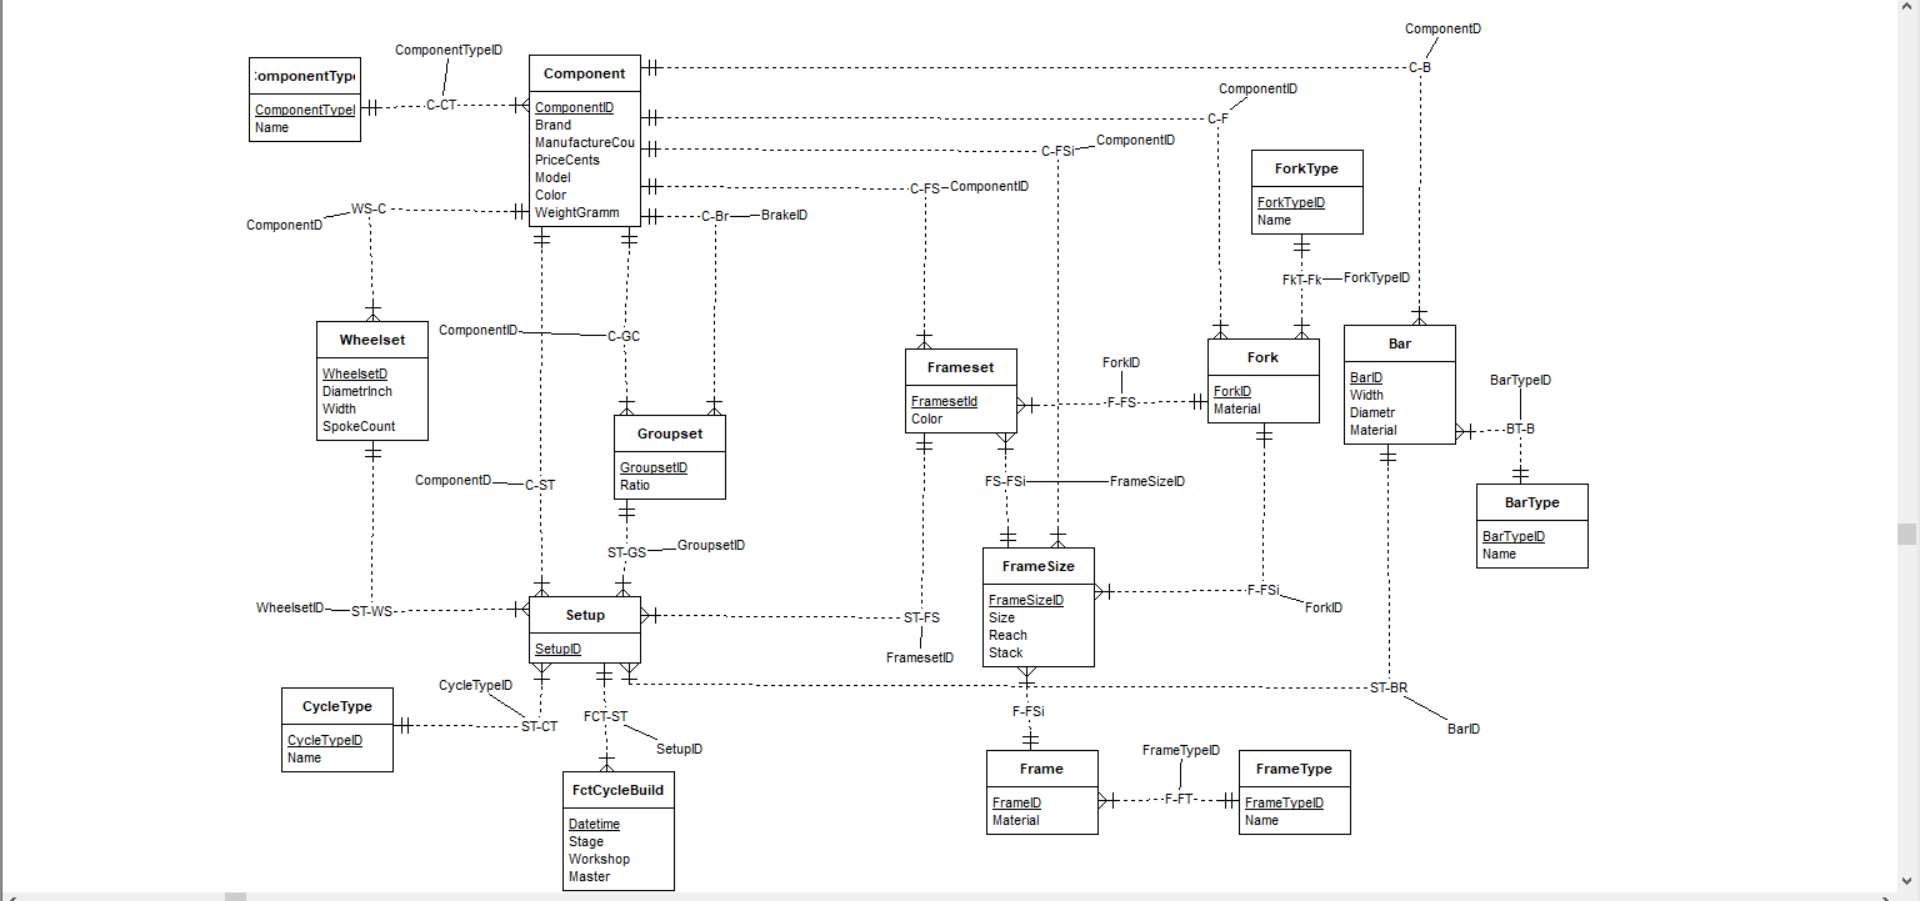
\includegraphics[width=1\linewidth]{1-cycle}
	\caption{Модель данных вело-предприятия}
	\label{fig:1-cycle}
\end{figure}



На данном этапе выполнения работы мы реализовали проект базы данных будущего хранилища данных, планируемого к применению в компании, занимающейся сборкой и поставкой велосипедов по индивидуальному заказу. Был проведен анализ переметной области, определен список сущностей, которые наиболее полно смогут описать сущности, участвующие в производственном процессе.
%%% Local Variables:
%%% mode: latex
%%% TeX-master: "rpz"
%%% End:

\newcommand{\erdatamodaler}{ERwin Data Modeler~}

\chapter{Создание логической и физической модели данных}
\label{cha:dmd}
В данном разделе будет рассмотрено создание логической и физической модели данных предложенных предметных областей в ПО ERwin Data Modeler.

На этапе инфологического проектирования базы данных должна быть построена
модель предметной области, не привязанная к конкретной СУБД, понятная не только
разработчикам информационной системы, но и экономистам, менеджерам и другим
специалистам. В то же время модель предметной области должна максимально точно
отражать семантику предметной области и позволять легко перейти к модели данных
конкретной СУБД.

\textbf{Логический уровень} --- это уровень, соответствующий инфологическому этапу проектирования
и не привязанный к конкретной СУБД. Модели логического уровня оперируют с
понятиями сущностей, атрибутов и связей, которые на этом уровне именуются на
естественном языке (в нашем случае – на русском) так, как они называются в
реальном мире.

\textbf{Физический уровень} --- это отображение логической модели на модель данных
конкретной СУБД. Одной логической модели может соответствовать несколько
физических моделей. Причем, Erwin (как и другие CASE-системы проектирования баз
данных) позволяет автоматизировать отображение логической модели на физическую.

\section{Работа по методическим указаниям}

Порядок построения модели данных в среде \erdatamodaler рассмотрим на примере
автоматизированной информационной системы <<Реализация средств вычислительной
техники>>, предназначенной для учета продаж настольных компьютеров по заказам
клиентов.

Создание модели данных начинается с разработки логической модели, которая
должна представлять состав сущностей предметной области с перечнем атрибутов и
отношений между ними.

Результат разработки логической модели данных системы <<Реализация средств
вычислительной техники>>, предназначенной для учета продаж настольных
компьютеров по заказам клиентов приведен на Рисунке \ref{fig:2-logical-model-method}.

% TODO: \usepackage{graphicx} required
\begin{figure}[htpb]
	\centering
	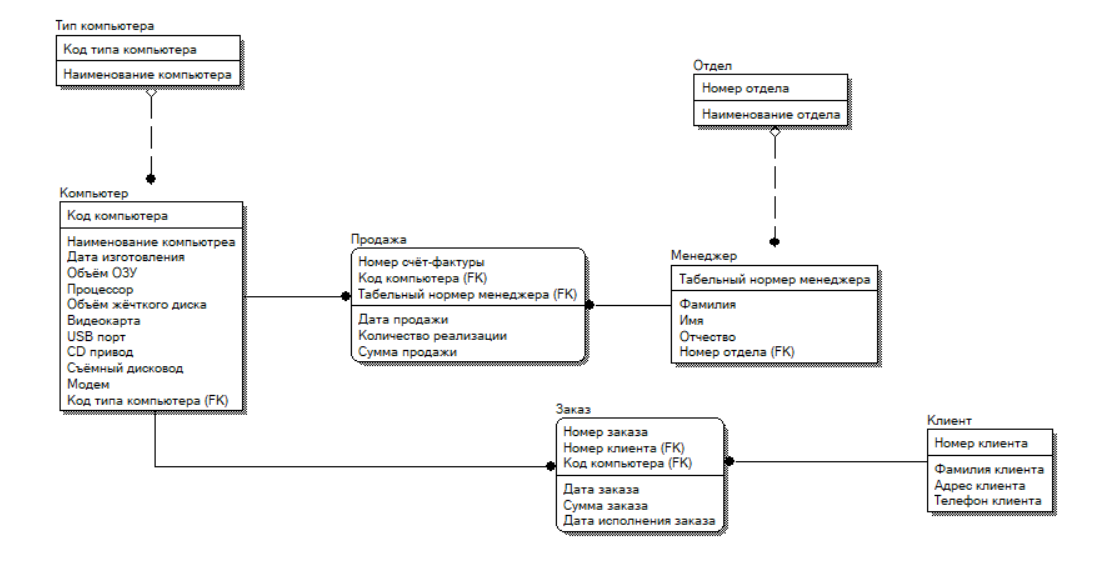
\includegraphics[angle=0,width=\linewidth]{/2-method}
	\caption{Логическая модель данных системы <<Реализация средств вычислительной техники>>}
	\label{fig:2-logical-model-method}
\end{figure}

Для построения физической модели данных системы, следует определиться с СУБД, в которой будет реализована модель. При построении физической модели данных следует учитывать формальную теория представления и обработки данных в конкретной системе управления базами данных (СУБД).

В данной практической работе в качестве СУБД выбрана MySQL.

Приступим к построению физической модели данных системы <<Реализация средств вычислительной техники>>. Результат работы можно видеть на Рисунке \ref{fig:2-phisical-model}.
%\newpage
% TODO: \usepackage{graphicx} required
\begin{figure}[ht]
	\centering
	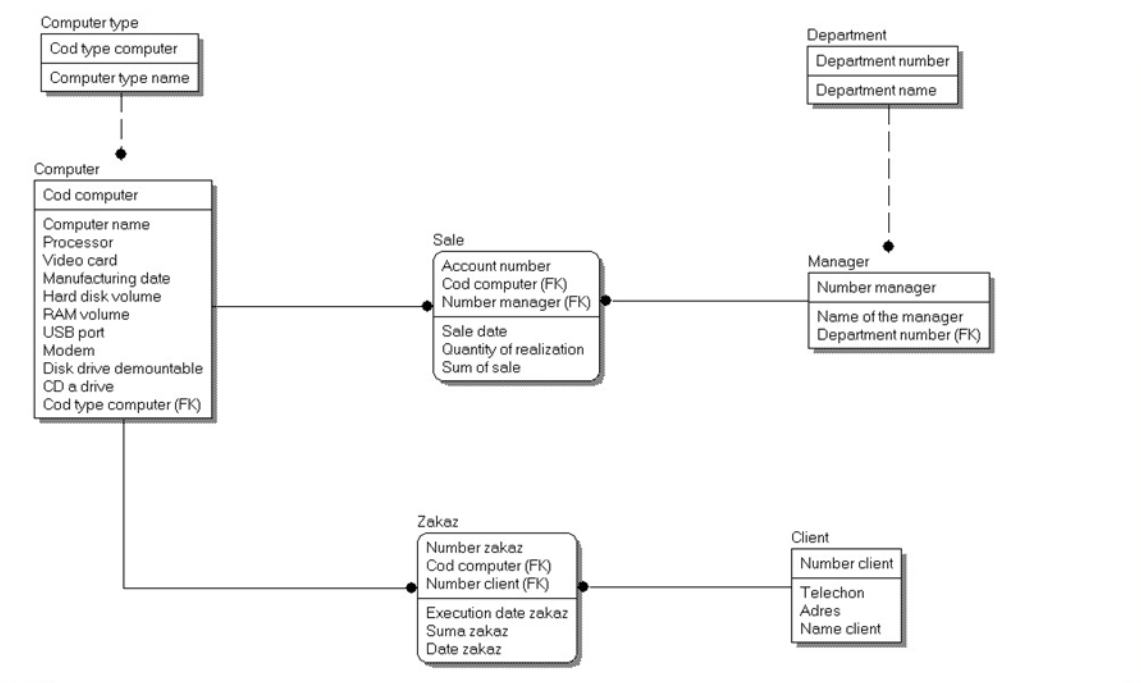
\includegraphics[angle=0,width=\linewidth]{2-phisical-model}
	\caption{Физическая модель данных системы <<Реализация средств вычислительной техники>>}
	\label{fig:2-phisical-model}
\end{figure}
\newpage
\subsection{Индивидуальное задание}
Приступим к построению логической модели данных системы <<Велосипедное предприятие>>. 
В соответствии с моделью, реализованной в ходе первой практической работы, добавим в рабочую область следующие сущности:
\begin{itemize}
	\item Component;
	\item FrameInfo;
	\item Frame;
	\item Frameset;
	\item FrameSize;
	\item Fork;
	\item ComponentType;
	\item Wheelset;
	\item Groupset;
	\item Brake;
	\item FctCycleBuild;
	\item CycleType;
	\item Bar;
	\item Setup.
\end{itemize}
Добавим связи между сущностями в соответствии с ранее построенной моделью. Логическая модель системы <<Велосипедное предприятие>> приведена на Рисунке \ref{fig:2-cycle-logical}.

% TODO: \usepackage{graphicx} required
\begin{figure}[h!]
	\centering
	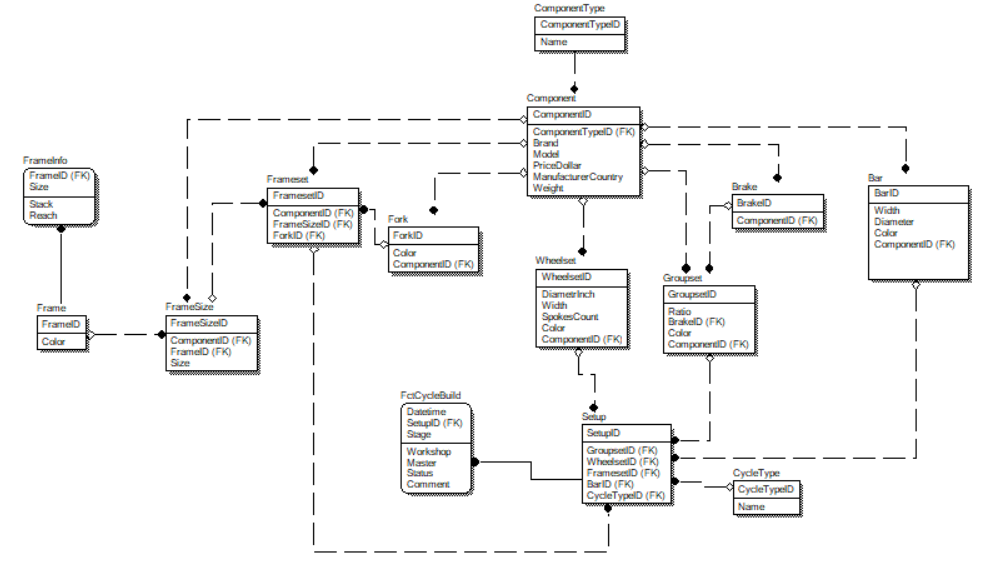
\includegraphics[width=0.8\linewidth]{2-cycle-logical}
	\caption{Логическая модель данных системы <<Велосипедное предприятие>>}
	\label{fig:2-cycle-logical}
\end{figure}

После уточнения типов данных, выбранных в соответствии с предметной областью и спецификой СУБД MySQL.
Физическая модель системы <<Велосипедное предприятие>> приведена на Рисунке \ref{fig:2-cycle-phisical}.

% TODO: \usepackage{graphicx} required
\begin{figure}[h!]
	\centering
	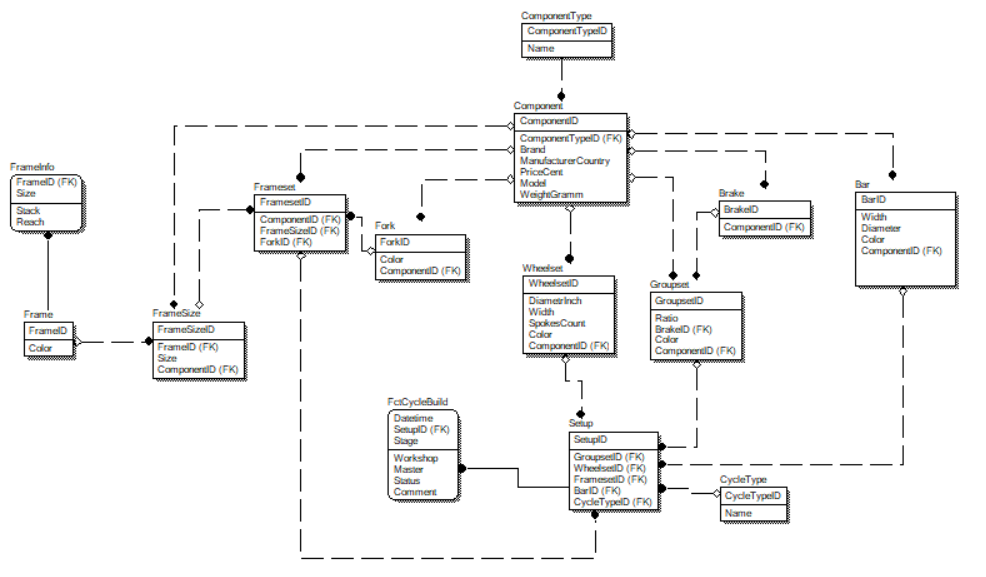
\includegraphics[width=0.8\linewidth]{2-cycle-phisical}
	\caption{Физическая модель данных системы <<Велосипедное предприятие>>}
	\label{fig:2-cycle-phisical}
\end{figure}

После реализации физической и логической модели можно приступать к реализации модели данной системы в СУБД MySQL.
\hfill
\chapter{Конструкторский раздел}
\label{cha:design}

В данном разделе проектируется новая всячина.

\section{Архитектура всячины}

\paragraph{Проверка} параграфа. Вроде работает.
\paragraph{Вторая проверка} параграфа. Опять работает.

Вот.

\begin{itemize}
\item Это список с <<палочками>>.
\item Хотя он и не по ГОСТ, кажется.
\end{itemize}

\begin{enumerate}
\item Поэтому для списка, начинающегося с заглавной буквы, лучше список с цифрами.
\end{enumerate}

Формула \ref{F:F1} совершено бессмысленна.

%Кстати, при каких-то условиях <<удавалось>> получить двойный скобки вокруг номеров формул. Вопрос исследуется.

\begin{equation}
a= cb
\label{F:F1}
\end{equation}


Окружение \texttt{cases} опять работает (см. \ref{F:F2}), спасибо И. Короткову за исправления..


\begin{equation}
a= \begin{cases}
 3x + 5y + z, \mbox{если хорошо} \\
 7x - 2y + 4z, \mbox{если плохо}\\
 -6x + 3y + 2z, \mbox{если совсем плохо}
\end{cases}
\label{F:F2}
\end{equation}

\section{Подсистема всякой ерунды}

Культурная вставка dot-файлов через утилиту dot2tex (рис.~\ref{fig:fig02}).

\begin{figure}
  \centering
% [width=0.5\textwidth] --- регулировка ширины картинки
  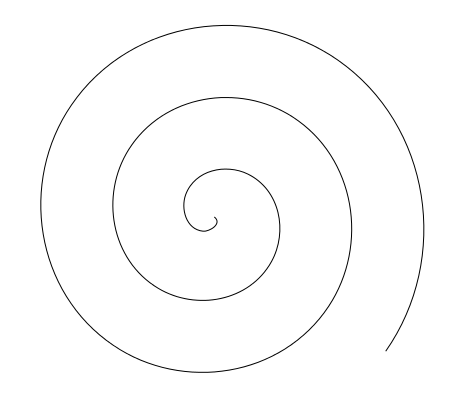
\includegraphics{figures/pic01}
  \caption{Рисунок}
  \label{fig:fig02}
\end{figure}


\subsection{Блок-схема всякой ерунды}

\subsubsection*{Кстати о заголовках}

У нас есть и \Code{subsubsection}. Только лучше её не нумеровать.

%%% Local Variables:
%%% mode: latex
%%% TeX-master: "rpz"
%%% End:

\chapter{Технологический раздел}
\label{cha:impl}

В данном разделе описано изготовление и требование всячины. Кстати,
в Latex нужно эскейпить подчёркивание (писать <<\verb|some\_function|>> для \Code{some\_function}).

\ifPDFTeX
Для вставки кода есть пакет \Code{listings}. К сожалению, пакет \Code{listings} всё ещё
работает криво при появлении в листинге русских букв и кодировке исходников utf-8.
В данном примере он (увы) на лету конвертируется в koi-8 в ходе сборки pdf.

Есть альтернатива \Code{listingsutf8}, однако она работает лишь с
\Code{\textbackslash{}lstinputlisting}, но не с окружением \Code{\textbackslash{}lstlisting}

Вот так можно вставлять псевдокод (питоноподобный язык определен в \Code{listings.inc.tex}):

\begin{lstlisting}[style=pseudocode,caption={Алгоритм оценки дипломных работ}]
def EvaluateDiplomas():
    for each student in Masters:
        student.Mark := 5
    for each student in Engineers:
        if Good(student):
            student.Mark := 5
        else:
            student.Mark := 4
\end{lstlisting}

Еще в шаблоне определен псевдоязык для BNF:

\begin{lstlisting}[style=grammar,basicstyle=\small,caption={Грамматика}]
  ifstmt -> "if" "(" expression ")" stmt |
            "if" "(" expression ")" stmt1 "else" stmt2
  number -> digit digit*
\end{lstlisting}

В листинге~\ref{lst:sample01} работают русские буквы. Сильная магия. Однако, работает
только во включаемых файлах, прямо в \TeX{} нельзя.

% Обратите внимание, что включается не ../src/..., а inc/src/...
% В Makefile есть соответствующее правило для inc/src/*,
% которое копирует исходные файлы из ../src и конвертирует из UTF-8 в KOI8-R.
% Кстати, поэтому использовать можно только русские буквы и ASCII,
% весь остальной UTF-8 вроде CJK и египетских иероглифов -- нельзя.

\lstinputlisting[language=C,caption=Пример (\Code{test.c}),label=lst:sample01]{listings/test.c}

\else

Для вставки кода есть пакет \texttt{minted}. Он хорош всем кроме: необходимости Python (есть во всех нормальных (нет, Windows, я не про тебя) ОС) и Pygments и того, что нормально работает лишь в \XeLaTeX.

Можно пользоваться расширенным BFN:

\begin{listing}[H]
\begin{ebnfcode}
 letter = "A" | "B" | "C" | "D" | "E" | "F" | "G"
       | "H" | "I" | "J" | "K" | "L" | "M" | "N"
       | "O" | "P" | "Q" | "R" | "S" | "T" | "U"
       | "V" | "W" | "X" | "Y" | "Z" ;
digit = "0" | "1" | "2" | "3" | "4" | "5" | "6" | "7" | "8" | "9" ;
symbol = "[" | "]" | "{" | "}" | "(" | ")" | "<" | ">"
       | "'" | '"' | "=" | "|" | "." | "," | ";" ;
character = letter | digit | symbol | "_" ;
 
identifier = letter , { letter | digit | "_" } ;
terminal = "'" , character , { character } , "'" 
         | '"' , character , { character } , '"' ;
 
lhs = identifier ;
rhs = identifier
     | terminal
     | "[" , rhs , "]"
     | "{" , rhs , "}"
     | "(" , rhs , ")"
     | rhs , "|" , rhs
     | rhs , "," , rhs ;
 
rule = lhs , "=" , rhs , ";" ;
grammar = { rule } ;
\end{ebnfcode}
\caption{EBNF определённый через EBNF}
\label{lst:ebnf}
\end{listing}

А вот в листинге \ref{lst:c} на языке C работают русские комменты. Спасибо Pygments и Minted за это.

\begin{listing}[H]
\cfile{inc/src/test.c}
\caption{Пример — test.c} 
\end{listing}
\label{lst:c}

\fi

% Для вставки реального кода лучше использовать \texttt{\textbackslash lstinputlisting} (который понимает
% UTF8) и стили \Code{realcode} либо \Code{simplecode} (в зависимости от размера куска).




Можно также использовать окружение \Code{verbatim}, если \Code{listings} чем-то не
устраивает. Только следует помнить, что табы в нём <<съедаются>>. Существует так же команда \Code{\textbackslash{}verbatiminput} для вставки файла.

\begin{verbatim}
a_b = a + b; // русский комментарий
if (a_b > 0)
    a_b = 0;
\end{verbatim}

%%% Local Variables:
%%% mode: latex
%%% TeX-master: "rpz"
%%% End:

\chapter{Экспериментальный раздел}
\label{cha:research}

В данном разделе проводятся вычислительные эксперименты.
А на рис.~\ref{fig:spire01} показана схема мыслительного процесса автора...

\begin{figure}
  \centering
  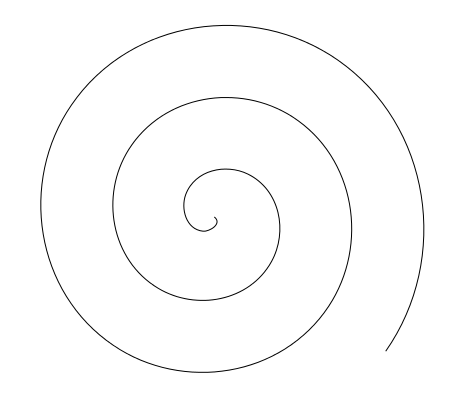
\includegraphics[width=\textwidth]{figures/pic01}
  \caption{Как страшно жить}
  \label{fig:spire01}
\end{figure}


%%% Local Variables:
%%% mode: latex
%%% TeX-master: "rpz"
%%% End:


\backmatter %% Здесь заканчивается нумерованная часть документа и начинаются ссылки и
            %% заключение

\Conclusion % заключение к отчёту

Результатом работы над данной курсовой работой является ознакомление с проблематикой разработки мультисинхронных устройств, реализация цифрового устройства ресинхронизации данных, представляющего собой асинхронную очередь данных, тактируемого двумя независимыми синхросигналами.

В ходе данной работы были проведены мероприятия по разработке функциональной и структурной схемы цифрового устройства и устройств, необходимых для его работы; созданию модуля, реализующего устройство ресинхронизации данных на языке описания аппаратуры Verilog; включению данного устройства в состав сложных устройств и проведение его отладки и тестирования.

Цели и задачи по реализации устройства для ресинхронизации данных выполнены. 

%%% Local Variables: 
%%% mode: latex
%%% TeX-master: "rpz"
%%% End: 


% % Список литературы при помощи BibTeX
% Юзать так:
%
% pdflatex rpz
% bibtex rpz
% pdflatex rpz

\bibliographystyle{gost780u}
\bibliography{course-scheme/rpz}

%%% Local Variables: 
%%% mode: latex
%%% TeX-master: "rpz"
%%% End: 


\appendix   % Тут идут приложения

\chapter{Картинки}
\label{cha:appendix1}

\begin{figure}
\centering
\caption{Картинка в приложении. Страшная и ужасная.}
\end{figure}

%%% Local Variables: 
%%% mode: latex
%%% TeX-master: "rpz"
%%% End: 

\chapter{Еще картинки}
\label{cha:appendix2}

\begin{figure}
\centering
\caption{Еще одна картинка, ничем не лучше предыдущей. Но надо же как-то заполнить место.}
\end{figure}

%%% Local Variables: 
%%% mode: latex
%%% TeX-master: "rpz"
%%% End: 


\end{document}

%%% Local Variables:
%%% mode: latex
%%% TeX-master: t
%%% End:
